\documentclass[../../main.tex]{subfiles}
\graphicspath{{../../image/}{../../figure/}}
\begin{document}

\section{用波曲线求解 Riemann 问题}\label{section:ch09-用波曲线求解riemann问题}

本节的目标是通过拼接常值状态、中心稀疏波与容许激波来构造 Riemann 问题的解。我们把研究限制在不同特征族的波速严格分离的情形。这既覆盖一般严格双曲方程组中小振幅波,也覆盖像\eqref{align:ch07-p系统}那样的特殊方程组中任意振幅的波,在那里所有 $1$-波向左传播,所有 $2$-波向右传播。

于是考虑一个有界变差的向外波扇\eqref{align:ch09-9-1-2}。按\cref{section:ch09-自相似解与riemann问题}中的讨论, $(-\infty,\infty)$ 被分解为激波集 $\mathscr{S}$、稀疏波集 $\mathscr{W}$ 与常值状态集 $\mathscr{C}$ 之并。由于不同特征族的波速严格分离, $\mathscr{S}=\bigcup_{i=1}^{n}\mathscr{S}_{i}$, $\mathscr{W}=\bigcup_{i=1}^{n}\mathscr{W}_{i}$,其中 $\mathscr{S}_{i}$ 是 $V$ 的 $i$-激波跳跃间断点(至多可数)集, $\mathscr{W}_{i}$ 是 $V$ 满足\eqref{align:ch09-9-1-7}的连续点(可能为空)集。集 $\mathscr{S}_{i}\cup\mathscr{W}_{i}$ 是闭的,并含有第 $i$ 特征族波速取值范围内的点。

现假定激波满足 Lax $E$ 条件,即对一切 $\xi\in\mathscr{S}_{i}$,
\begin{align}
\lambda_{i}(V(\xi+))\leqslant\xi\leqslant\lambda_{i}(V(\xi-)).
\label{align:ch09-9-3-1}
\end{align}
则 $\mathscr{S}_{i}\cup\mathscr{W}_{i}$ 必为闭区间 $[\zeta_{i},\xi_{i}]$。事实上,设 $\mathscr{S}_{i}\cup\mathscr{W}_{i}$ 不连通。则存在开区间 $(\zeta,\xi)\subset\mathscr{C}$,其端点 $\zeta,\xi\in\mathscr{S}_{i}\cup\mathscr{W}_{i}$。特别地, $V(\zeta+)=V(\xi-)$。另一方面,由\eqref{align:ch09-9-1-7}与\eqref{align:ch09-9-3-1}, $\zeta\geqslant\lambda_{i}(V(\zeta+))$, $\xi\leqslant\lambda_{i}(V(\xi-))$,与 $\zeta<\xi$ 矛盾。还注意到,任一满足 $\xi>\zeta_{i}$(或 $\xi<\xi_{i}$)的 $\xi\in\mathscr{S}_{i}$ 是 $\mathscr{W}_{i}$ 中点的递增(或递减)序列的极限,故 $\lambda_{i}(V(\xi-))=\xi$(或 $\lambda_{i}(V(\xi+))=\xi$)。于是我们建立了如下

\begin{theorem}\label{theorem:ch09-波扇结构}
假定不同特征族的波速严格分离。Riemann 问题\eqref{align:ch09-9-1-1}、\eqref{align:ch09-9-1-18}的任一自相似解\eqref{align:ch09-9-1-2}(其激波满足 Lax $E$ 条件)由 $n+1$ 个常值状态 $U_{L}=U_{0},U_{1},\dots,U_{n-1},U_{n}=U_{R}$ 组成。对 $i=1,\dots,n$, $U_{i-1}$ 与 $U_{i}$ 由一个 $i$-波连接,即一串中心 $i$-稀疏波和/或 $i$-激波,其性质为:左侧(和/或右侧)以 $i$-稀疏波为界的 $i$-激波是左(和/或右) $i$-接触间断(见\cref{figure:ch09-波扇})。
\end{theorem}

单个 $i$-激波与单个 $i$-稀疏波称为\emph{初等 $i$-波}。当需要回忆或强调 $i$-波可能含有不止一个初等 $i$-波时,使用术语\emph{复合 $i$-波}。

\begin{figure}[ht]
\centering
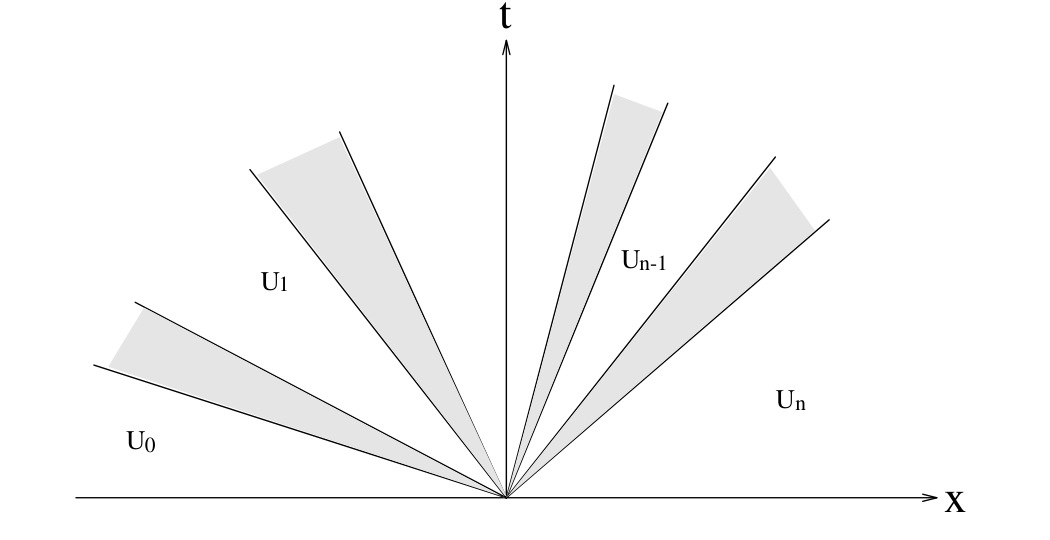
\includegraphics[width=0.75\textwidth]{ch09-fig03-01.png}
\caption{由 $n$ 个波组成的向外波扇,常值状态为 $U_{0},U_{1},\dots,U_{n}$。}
\label{figure:ch09-波扇}
\end{figure}

接下来两节将证明:可在固定状态 $\bar{U}\in\mathscr{O}$ 的右侧(或左侧)由一个容许 $i$-波(由 $i$-稀疏波与容许 $i$-激波组成)连接到的状态轨迹,是一条 Lipschitz 曲线 $\Phi_{i}(\tau;\bar{U})$(或 $\Psi_{i}(\tau;\bar{U})$),称为过 $\bar{U}$ 的\emph{前向}(或\emph{后向})\emph{$i$-波曲线},它可参数化为
\begin{align}
\Phi_{i}(\tau;\bar{U})=\bar{U}+\tau R_{i}(\bar{U})+P_{i}(\tau;\bar{U}),
\label{align:ch09-9-3-2}
\end{align}
\begin{align}
\Psi_{i}(\tau;\bar{U})=\bar{U}+\tau R_{i}(\bar{U})+Q_{i}(\tau;\bar{U}),
\label{align:ch09-9-3-3}
\end{align}
其中 $P_{i}$、$Q_{i}$ 是 $(\tau,U)$ 的 Lipschitz 连续函数,在 $\tau=0$ 处为零;当 $\tau$ 限制在原点充分小邻域内时,其 Lipschitz 常数可任意小。

暂时把上述性质的波曲线的存在性视为已知,我们注意到:要求解 Riemann 问题,须确定一个 $n$-元组 $\varepsilon=(\varepsilon_{1},\dots,\varepsilon_{n})$,视为 $\mathbb{R}^{n}$ 中的点,使得从 $U_{0}=U_{L}$ 出发依次计算 $U_{i}=\Phi_{i}(\varepsilon_{i};U_{i-1})$, $i=1,\dots,n$,最终得到 $U_{n}=U_{R}$。据此我们定义函数
\begin{align}
\Omega(\varepsilon;\bar{U})=\Phi_{n}(\varepsilon_{n};\Phi_{n-1}(\varepsilon_{n-1};\cdots\Phi_{1}(\varepsilon_{1};\bar{U})\cdots)).
\label{align:ch09-9-3-4}
\end{align}
显然,
\begin{align}
\Omega(\varepsilon;\bar{U})=\bar{U}+\sum_{i=1}^{n}\varepsilon_{i}R_{i}(\bar{U})+G(\varepsilon;\bar{U}),
\label{align:ch09-9-3-5}
\end{align}
其中 $G$ 是 Lipschitz 函数,在 $\varepsilon=0$ 处为零;当 $\varepsilon$ 限制在原点充分小邻域内时,其 Lipschitz 常数可任意小。当 $U_{R}$ 充分接近 $U_{L}$ 时,存在唯一的充分小 $\varepsilon$ 使 $\Omega(\varepsilon;U_{L})=U_{R}$。事实上,此 $\varepsilon$ 可通过如下迭代格式构造:取 $\varepsilon^{(0)}=0$,对 $m=1,2,\dots$,
\begin{align}
\varepsilon_{i}^{(m)}=L_{i}(U_{L})[U_{R}-U_{L}]-L_{i}(U_{L})G(\varepsilon^{(m-1)};U_{L}),\qquad i=1,\dots,n,
\label{align:ch09-9-3-6}
\end{align}
由显然的压缩论证知其收敛。这生成 Riemann 问题的一个解,在有中等强度波的自相似解类中唯一。连接 $U_{L}$ 与 $U_{R}$ 的波扇可方便地由其左状态 $U_{L}$ 与 $n$-元组 $\varepsilon=(\varepsilon_{1},\dots,\varepsilon_{n})$ 标识。$\varepsilon_{i}$ 的值确定 $i$-波振幅,而 $|\varepsilon_{i}|$ 度量 $i$-波强度。

在 $\Phi_{i}$ 为 $C^{2,1}$ 的特殊情形,我们将看到
\begin{align}
\dot{\Phi}_{i}(0;\bar{U})=R_{i}(\bar{U}),\qquad\ddot{\Phi}_{i}(0;\bar{U})=\mathrm{D}R_{i}(\bar{U})R_{i}(\bar{U}).
\label{align:ch09-9-3-7}
\end{align}
于是 $\Omega$ 也是 $C^{2,1}$。由于 $\Omega(0,\dots,0,\varepsilon_{i},0,\dots,0;\bar{U})=\Phi_{i}(\varepsilon_{i};\bar{U})$,
\begin{align}
\frac{\partial\Omega}{\partial\varepsilon_{i}}(0;\bar{U})=R_{i}(\bar{U}),\qquad 1\leqslant i\leqslant n,
\label{align:ch09-9-3-8}
\end{align}
\begin{align}
\frac{\partial^{2}\Omega}{\partial\varepsilon_{i}^{2}}(0;\bar{U})=\mathrm{D}R_{i}(\bar{U})R_{i}(\bar{U}),\qquad 1\leqslant i\leqslant n.
\label{align:ch09-9-3-9}
\end{align}
此外,当 $j<k$ 时, $\Omega(0,\dots,0,\varepsilon_{j},0,\dots,0,\varepsilon_{k},0,\dots,0;\bar{U})=\Phi_{k}(\varepsilon_{k};\Phi_{j}(\varepsilon_{j};\bar{U}))$,故
\begin{align}
\frac{\partial^{2}\Omega}{\partial\varepsilon_{j}\partial\varepsilon_{k}}(0;\bar{U})=\mathrm{D}R_{k}(\bar{U})R_{j}(\bar{U}),\qquad 1\leqslant j<k\leqslant n.
\label{align:ch09-9-3-10}
\end{align}
由\eqref{align:ch09-9-3-8}、\eqref{align:ch09-9-3-9}与\eqref{align:ch09-9-3-10},
\begin{align}
U_{R}&=U_{L}+\sum_{i=1}^{n}\varepsilon_{i}R_{i}(U_{L})+\tfrac{1}{2}\sum_{i=1}^{n}\varepsilon_{i}^{2}\mathrm{D}R_{i}(U_{L})R_{i}(U_{L})
\nonumber\\
&\quad+\sum_{j=1}^{n}\sum_{k=j+1}^{n}\varepsilon_{j}\varepsilon_{k}\mathrm{D}R_{k}(U_{L})R_{j}(U_{L})+O(|\varepsilon|^{3}).
\label{align:ch09-9-3-11}
\end{align}

显然,我们也可以按相反顺序合成 Riemann 问题的解:从 $U_{n}=U_{R}$ 出发,依次计算状态 $U_{i-1}=\Psi_{i}(\varepsilon_{i};U_{i})$, $i=n,\dots,1$,直到到达 $U_{0}=U_{L}$。在某些情形下,混合策略可能是有利的。例如,对 $n=2$ 的两个守恒律方程组求解 Riemann 问题,最有效的做法是:过左状态 $U_{L}$ 画前向 $1$-波曲线 $\Phi_{1}(\varepsilon_{1};U_{L})$,过右状态 $U_{R}$ 画后向 $2$-波曲线 $\Psi_{2}(\varepsilon_{2};U_{R})$。这两条曲线的交点确定中间常值状态: $U_{M}=\Phi_{1}(\varepsilon_{1};U_{L})=\Psi_{2}(\varepsilon_{2};U_{R})$。

\end{document}
